\documentclass[journal]{IEEEtran}

\usepackage[utf8]{inputenc}
\usepackage[T1]{fontenc}
\usepackage{amsmath,amssymb,amsfonts}
\usepackage{algorithm}
\usepackage{algpseudocode}
\usepackage{graphicx}

\usepackage{booktabs}
\usepackage{makecell}
\usepackage{multirow}
\usepackage{url}
\usepackage{hyperref}
\usepackage{tikz}
\usepackage{pgfplots}
\pgfplotsset{compat=1.17}
\usetikzlibrary{arrows.meta, positioning, calc, shapes.geometric}
\usepackage{cite}
\usepackage{xcolor}

\hyphenation{op-tical net-works semi-conduc-tor}

\begin{document}

\title{TAFS: Transformer-Attentive Feature Selection for Sequential Regression}
\author{Huseyin~Karaca$^{*}$,
        A.~Samil~Namli$^{*}$, 
        and Suleyman S.~Kozat,~\IEEEmembership{Senior~Member,~IEEE}
\thanks{$^{*}$H. Karaca and A. S. Namli contributed equally to this work.}
\thanks{H. Karaca, A. S. Namli, and S. S. Kozat are with Bilkent University, Ankara, Turkiye. H. Karaca and A. S. Namli are also with Turk Telekom, Ankara, Turkiye (e-mails: \{huseyin.karaca, samil.namli\}@bilkent.edu.tr; kozat@ee.bilkent.edu.tr).}%
\thanks{This work is supported by The Scientific and Technological Research Council of Turkiye (TUBITAK) 1515 Frontier R\&D Laboratories Support Program for Turk Telekom 6G R\&D Lab under project number 5249902, and by the TUBITAK 2210-A program.}%
}
% \markboth{Preprint -- TAFS}{Anonymous: TAFS}
\markboth{Draft, \today}{TAFS: Transformer-Attentive Feature Selection for Sequential Regression}

\maketitle

\begin{abstract}
This article addresses one-step sequential regression in regimes where the input is a high-dimensional vector of engineered features and the underlying data-generating process is non-stationary. In this setting, a fixed pool of pretrained base forecasters covers complementary regions of the input space, and the operational question is how to combine them in a manner that tracks the time-varying importance of the features. We introduce TAFS, a framework that treats each engineered feature as a token, processes it with a feature-axis transformer conditioned on a context summary of the recent history, and reads out combination weights over the base forecasters under one of three constraint regimes (unconstrained, affine, convex). The attention weights produced by the transformer provide a per-feature importance signal, and the pipeline is trained end-to-end on cumulative prediction error. On a controlled synthetic regime-switch task, TAFS approaches the per-step oracle and lowers prediction error by $41\%$ relative to a context-free variant whose attention mechanism cannot adapt to regime changes. On the Istanbul Stock Exchange benchmark, TAFS attains the best overall performance with a MASE of $0.252$, yielding a $56\%$ reduction relative to the strongest competing learned ensemble and a $7\%$ improvement over the best individual predictor. On a more challenging Exchange-Rate return series that exhibits near-random-walk behavior, TAFS remains competitive while continuing to outperform simple averaging, the best validation-selected single predictor, and all static-transform baselines. Throughout, inference cost remains dominated by the cached base predictions, to which the transformer adds only a small overhead.
% We also discuss a short convergence argument for the smooth-loss case.
\end{abstract}

\begin{IEEEkeywords}
Time-series forecasting, feature selection, transformers, attention, meta-learning, ensemble of forecasters.
\end{IEEEkeywords}

\section{Introduction}

\subsection{Background}

Sequential regression problems arising in energy demand forecasting, financial return prediction, retail sales planning and meteorology require the construction of several hundred engineered features (lags, rolling statistics, calendar variables, exogenous series) from several hundred to several thousand observations~\cite{box2015tsbook,makridakis2020m4,makridakis2022m5}. In this regime no single forecaster is uniformly optimal. Gradient-boosted decision trees~\cite{ke2017lightgbm,chen2016xgboost,prokhorenkova2018catboost} and regularised linear models~\cite{tibshirani1996lasso} are accurate on tabular features; recurrent~\cite{hochreiter1997lstm,salinas2020deepar} and basis-expansion networks~\cite{oreshkin2020nbeats} capture longer dependencies; classical state-space models such as SARIMAX~\cite{box2015tsbook} model seasonality. The relative ranking of these models varies both across datasets and across regimes \emph{within} a single dataset.

The relevance of an individual engineered feature is also time-varying. A demand series dominated by a weekly cycle in one quarter may shift to being dominated by a holiday calendar in another; an exchange rate driven by an interest-rate differential under one monetary regime may transition to being driven by trade-balance shocks under another. Static feature-selection pipelines, whether filter, wrapper, or embedded~\cite{guyon2003introfs,kononenko1994relieff}, fix the selection at training time and cannot react to such shifts. Static learned feature transforms address this only partially: a diagonal gate, a linear projection or a low-rank bottleneck can sharpen the relevant directions on average, but those directions remain fixed once training terminates.

\subsection{Related Work}

% \textbf{Feature selection and learned feature transforms.} 
Filter methods such as Pearson correlation and mutual-information ranking~\cite{cover1991ifs}, wrapper methods such as forward/backward selection~\cite{guyon2003introfs} and embedded methods such as Lasso~\cite{tibshirani1996lasso} or tree-based importance~\cite{breiman2001randomforest} all collapse the relevance signal to a single, dataset-level score. Learned feature transforms attached to a downstream selector or regressor improve over this by adapting the geometry of the feature space to the supervised objective; popular parameterizations are diagonal gating, full linear projections, low-rank bottlenecks, and small nonlinear MLPs. These transforms are static: once the parameters are estimated, the same map is applied at every time step.

% \textbf{Combining forecasters.}
Combining several forecasters with learned weights is a well-established methodology, with stacking~\cite{wolpert1992stacking,breiman1996stacked} as the canonical instance and time-varying weighting schemes as recurring refinements~\cite{vilalta2002metalearning}. Mixture-of-experts gating~\cite{jacobs1991moe,shazeer2017moe} produces input-conditional weights through a soft gate, and recent work applies MoE formulations to forecasting~\cite{shi2024timemoe}. Such combiners operate on a fixed feature representation; they do not modulate which features the downstream predictor consumes.

% \textbf{Transformers for time series.} 
Transformers~\cite{vaswani2017attention} have been adapted to forecasting along two axes: (i) the time axis, with sparse or decomposition-based attention~\cite{zhou2021informer,wu2021autoformer}, and (ii) the variable axis, where each variable becomes a token~\cite{liu2024itransformer,nie2023patchtst}. Linear baselines remain accurate on standard benchmarks~\cite{zeng2023dlinear}, indicating that the benefit of attention is in adaptivity rather than in raw capacity. Interpretable variants such as the Temporal Fusion Transformer~\cite{lim2021tft} expose per-feature importance through variable-selection networks; the importance there is produced by an independent gating subnetwork rather than by the attention mechanism that drives the downstream prediction.

% \textbf{Position of this work.} 
TAFS combines three ingredients that have appeared separately in the literature but, to our knowledge, not together: (i) a feature-axis transformer whose own attention mass on each feature token is the time-varying importance signal; (ii) a context token, derived from the recent target history and from regime indicators, that conditions this attention on the local state of the series; and (iii) a constrained combination head that maps the transformer output to weights over a pool of pretrained base forecasters, under unconstrained, affine, or convex regimes. The whole pipeline is trained end-to-end on cumulative prediction error, and the base forecasters are kept frozen so that inference cost remains close to running them once.

\subsection{Contributions}

\begin{itemize}
\item We introduce TAFS, a framework for sequential regression that performs joint, time-varying feature selection and forecaster combination through a feature-axis transformer with context conditioning.
\item We show that the four most common static feature transforms (diagonal, linear, low-rank, nonlinear) are limiting cases of the proposed attention map and are recovered when the context token is removed and the attention is restricted; this makes TAFS a strict superset.
\item We propose three combination-head variants (unconstrained, affine, convex), discuss when each is preferable. 
%, and give a short stationary-point argument for the smooth-loss training objective in Appendix~\ref{app:convergence}.
\item We evaluate TAFS on a controlled synthetic regime-switch task and on two real financial datasets (the Istanbul Stock Exchange index and a daily Exchange-Rate series), against baselines that include individual forecasters, conventional ensembles, four static learned transforms, and two meta-learners without feature selection. On the synthetic task, TAFS reduces prediction error by $41\%$ relative to a context-free variant. On the Istanbul Stock Exchange benchmark, it achieves the best overall MASE of $0.252$, improving by $56\%$ over the strongest competing learned ensemble and by $7\%$ over the best individual predictor. On the near-random-walk Exchange-Rate returns, it remains competitive while improving on simple averaging, the validation-selected best single predictor, and every static-transform baseline.

\item We release the full reproducibility package, including source code, training configurations, and dataset preprocessing pipelines, at \url{https://github.com/huseyin-karaca/tafs}.
\end{itemize}

\subsection{Organization}
The remainder of this article is organized as follows. Section~\ref{sec:problem} formalises the problem. Section~\ref{sec:method} describes the architecture and the training procedure. Section~\ref{sec:experiments} reports the synthetic study, the real-data comparison and the ablations. Section~\ref{sec:conclusion} concludes.
% Appendix~\ref{app:convergence} sketches the convergence argument.

\section{Problem Definition}
\label{sec:problem}

We consider a univariate sequential regression problem with exogenous covariates. At each time step $t = 1,\dots,T$ the target $y_t \in \mathbb{R}$ is observed together with a vector of engineered features $\mathbf{x}_t \in \mathbb{R}^p$ built from lags of $y$, rolling statistics, calendar variables and exogenous series. We assume a fixed pool of $K$ pretrained base forecasters
\[
\mathcal{F} = \{f_1, f_2, \dots, f_K\},
\]
each of which produces a one-step prediction $\hat{y}^{(k)}_t = f_k(\mathbf{x}_t)$ from the same $\mathbf{x}_t$.\footnote{The framework supports multi-step forecasting unchanged; we treat the $H$-step prediction as a vector and average the loss over the horizon. We keep the one-step notation for clarity.} The base predictions are computed offline and cached.

Let $\boldsymbol{\hat{y}}_t = \bigl(\hat{y}^{(1)}_t,\dots,\hat{y}^{(K)}_t\bigr)^\top \in \mathbb{R}^K$. A combination policy is a function $\pi_\theta$ that takes $\mathbf{x}_t$ together with a context summary $\mathbf{s}_t \in \mathbb{R}^{d_c}$ and returns a weight vector
\[
\mathbf{w}_t = \pi_\theta(\mathbf{x}_t, \mathbf{s}_t) \in \mathcal{W} \subseteq \mathbb{R}^K,
\]
where the admissible set $\mathcal{W}$ encodes one of three constraint regimes:
\begin{align}
\mathcal{W}_{\mathrm{u}}      &= \mathbb{R}^K,\\
\mathcal{W}_{\mathrm{a}}      &= \{\mathbf{w} \in \mathbb{R}^K : \mathbf{1}^\top \mathbf{w} = 1\},\\
\mathcal{W}_{\mathrm{c}}      &= \{\mathbf{w} \in \mathbb{R}^K_{\ge 0} : \mathbf{1}^\top \mathbf{w} = 1\}.
\end{align}
The combined prediction is $\tilde{y}_t = \mathbf{w}_t^\top \boldsymbol{\hat{y}}_t$. Given a per-step loss $\ell : \mathbb{R} \times \mathbb{R} \to \mathbb{R}_{\ge 0}$ (squared, Huber, or pinball), training minimises the cumulative loss
\begin{equation}
\label{eq:cumloss}
\mathcal{L}(\theta) \;=\; \frac{1}{T} \sum_{t=1}^{T} \ell\!\bigl(y_t,\, \pi_\theta(\mathbf{x}_t, \mathbf{s}_t)^\top \boldsymbol{\hat{y}}_t\bigr).
\end{equation}

In the regime of interest $p$ is typically large (tens to several hundred), $T$ is moderate (several hundred to several thousand), and the conditional importance of features in $\mathbf{x}_t$ for predicting $y_t$ is non-stationary in $t$. Selection mechanisms that compress $\mathbf{x}_t$ into a single static map discard this temporal structure and plateau above the per-step oracle, $\mathbf{w}_t^\star = \mathbf{e}_{\arg\min_k \ell(y_t,\hat{y}^{(k)}_t)}$.

\section{Proposed Work}
\label{sec:method}

We instantiate $\pi_\theta$ as a feature-axis transformer with context conditioning, followed by a constraint-aware combination head. An overview is given in Figure~\ref{fig:architecture}.

\begin{figure*}[t]
\centering
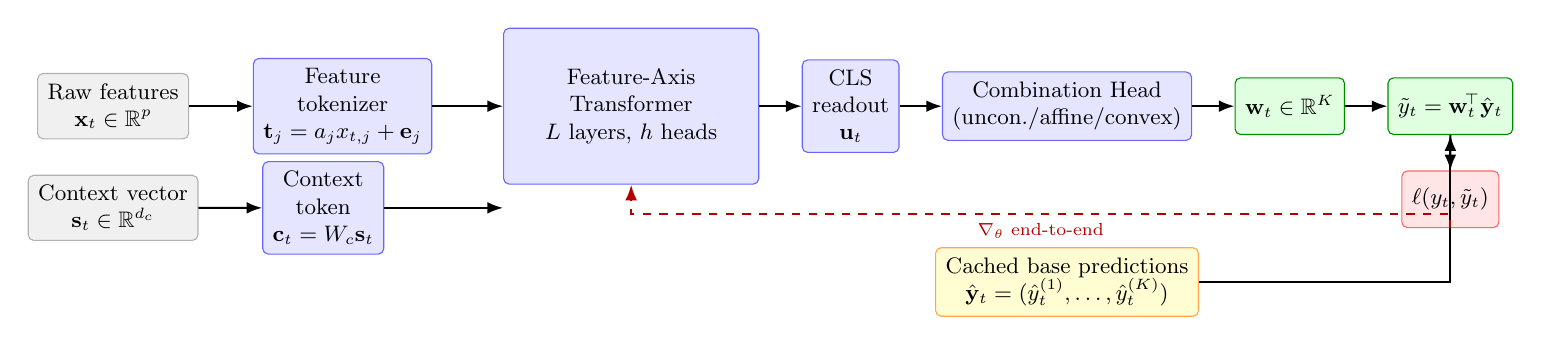
\begin{tikzpicture}[
    transform shape, % Scales nodes along with coordinates
    scale=0.9,       % Adjust this value (e.g., 0.85 to 0.95) to dial in the perfect fit
    node distance=0.4cm and 0.5cm, % Slightly tightens the global spacing between nodes
    font=\small,
    nbox/.style={draw, rounded corners=2pt, minimum height=0.8cm, align=center, inner sep=4pt},
    frozen/.style={nbox, fill=gray!12, draw=gray!60},
    learn/.style={nbox, fill=blue!10, draw=blue!60},
    nout/.style={nbox, fill=green!12, draw=green!55!black},
    cache/.style={nbox, fill=yellow!18, draw=orange!70},
    arr/.style={-{Latex[length=2mm]}, thick}
]
% Inputs
\node[frozen] (xt) at (0, 0) {Raw features\\$\mathbf{x}_t \in \mathbb{R}^p$};
\node[frozen, below=0.5cm of xt] (ct) {Context vector\\$\mathbf{s}_t \in \mathbb{R}^{d_c}$};

% Tokenization
\node[learn, right=0.9cm of xt] (tok) {Feature\\tokenizer\\$\mathbf{t}_j = a_j x_{t,j} + \mathbf{e}_j$};

% Context token
\node[learn, right=0.9cm of ct] (ctok) {Context\\token\\$\mathbf{c}_t = W_c \mathbf{s}_t$};

% Transformer block
\node[learn, right=1.0cm of tok, minimum width=3.6cm, minimum height=2.2cm] (tr) {Feature-Axis\\Transformer\\$L$ layers, $h$ heads};

% Pool
\node[learn, right=0.6cm of tr] (pool) {CLS\\readout\\$\mathbf{u}_t$};

% Constraint head
\node[learn, right=0.6cm of pool, minimum width=2.6cm] (head) {Combination Head\\(uncon./affine/convex)};

% Output weights
\node[nout, right=0.6cm of head] (wt) {$\mathbf{w}_t \in \mathbb{R}^K$};

% Base predictors
\node[cache, below=1.5cm of head] (yhat) {Cached base predictions\\$\hat{\mathbf{y}}_t = (\hat{y}^{(1)}_t,\dots,\hat{y}^{(K)}_t)$};

% Final
\node[nout, right=0.6cm of wt] (final) {$\tilde{y}_t = \mathbf{w}_t^{\!\top}\hat{\mathbf{y}}_t$};

% Loss
\node[nbox, fill=red!10, draw=red!60, below=0.5cm of final] (loss) {$\ell(y_t, \tilde{y}_t)$};

% Arrows
\draw[arr] (xt) -- (tok);
\draw[arr] (ct) -- (ctok);
\draw[arr] (tok) -- (tr.west |- tok);
\draw[arr] (ctok) -- (tr.west |- ctok);
\draw[arr] (tr) -- (pool);
\draw[arr] (pool) -- (head);
\draw[arr] (head) -- (wt);
\draw[arr] (wt) -- (final);
\draw[arr] (yhat) -| (final);
\draw[arr] (final) -- (loss);

% Backprop dashed arrow
% \draw[arr, dashed, red!70!black, bend right=20] (loss.west) to node[midway, below, font=\scriptsize]{$\nabla_\theta$ end-to-end} (tr.south);
\draw[arr, dashed, red!70!black] (loss.south) -- ++(0,+0.2cm) -| node[pos=0.25, below, font=\scriptsize]{$\nabla_\theta$ end-to-end} (tr.south);

\end{tikzpicture}
\caption{Overview of the proposed TAFS framework. Each of the $p$ engineered features is treated as a token with a learnable identity embedding, and a context token derived from lagged targets and regime indicators is prepended. A feature-axis transformer produces a task-aligned summary $\mathbf{u}_t$, which is mapped by a combination head to weights $\mathbf{w}_t$ over $K$ pretrained base forecasters under one of three constraint regimes (unconstrained, affine, convex). The final prediction is a weighted sum of cached base outputs $\hat{\mathbf{y}}_t$, and the cumulative prediction error is back-propagated end-to-end through the transformer and the head; base predictors are kept frozen.}
\label{fig:architecture}
\end{figure*}


\subsection{Feature-Axis Tokenization}
\label{sec:features}

The transformer treats each of the $p$ engineered features as a separate token in a sequence of length $p$. For feature $j$ at time $t$, the input token is
\begin{equation}
\mathbf{t}_{t,j} \;=\; a_j \cdot x_{t,j} \;+\; \mathbf{e}_j \;\in\; \mathbb{R}^d,
\end{equation}
where $a_j \in \mathbb{R}^d$ is a learnable scaling vector that lifts the scalar feature value into the model dimension $d$, and $\mathbf{e}_j \in \mathbb{R}^d$ is a learnable feature-identity embedding. Features are organised into named families (lags, rollings, calendar, exogenous, regime indicators); to encourage early structure during training we initialise $\mathbf{e}_j$ to a family-specific anchor plus small Gaussian noise.

Before applying the transformer we prepend two extra tokens. The first is a CLS token $\mathbf{c}_\mathrm{cls} \in \mathbb{R}^d$, used as the readout for the combination head; the second is a context token $\mathbf{c}_t = W_c \mathbf{s}_t + \mathbf{b}_c$, where $\mathbf{s}_t$ stacks (a) the most recent $L_y$ lags of $y$, (b) the residuals of $y_t$ against a simple seasonal-na\"ive predictor, and (c) optional regime indicators (e.g.\ binary flags for trading vs.\ non-trading days). The input sequence to the transformer is
\begin{equation}
\mathbf{Z}_t^{(0)} \;=\; (\mathbf{c}_\mathrm{cls},\, \mathbf{c}_t,\, \mathbf{t}_{t,1},\, \mathbf{t}_{t,2},\, \dots,\, \mathbf{t}_{t,p}) \;\in\; \mathbb{R}^{(p+2)\times d}.
\end{equation}

\subsection{Feature-Axis Transformer}

We apply a stack of $L$ pre-norm transformer encoder layers~\cite{vaswani2017attention} with $h$ heads, hidden width $d$, and feed-forward width $d_{\mathrm{ffn}}$:
\begin{align}
\mathbf{Z}_t^{(\ell+\tfrac{1}{2})} &= \mathbf{Z}_t^{(\ell)} + \mathrm{MHA}\!\bigl(\mathrm{LN}(\mathbf{Z}_t^{(\ell)})\bigr),\\
\mathbf{Z}_t^{(\ell+1)} &= \mathbf{Z}_t^{(\ell+\tfrac{1}{2})} + \mathrm{FFN}\!\bigl(\mathrm{LN}(\mathbf{Z}_t^{(\ell+\tfrac{1}{2})})\bigr).
\end{align}
No positional encoding is added: the feature axis is permutation-invariant, and the identity embeddings $\mathbf{e}_j$ already encode which token corresponds to which feature.

The output of the final layer is $\mathbf{Z}_t^{(L)} \in \mathbb{R}^{(p+2)\times d}$. We define
\begin{equation}
\mathbf{u}_t \;=\; \mathbf{Z}_t^{(L)}[0,:] \;\in\; \mathbb{R}^d
\end{equation}
as the task-aligned summary read from the CLS position. We also keep the per-feature attention weights $A^{(\ell,m)}_{0,j+2}$ from the CLS token to each feature token $j$ at layer $\ell$ and head $m$ for interpretation; averaged over layers and heads they give a single feature-importance score per step,
\begin{equation}
\label{eq:alpha}
\alpha_{t,j} \;=\; \frac{1}{Lh} \sum_{\ell=1}^{L} \sum_{m=1}^{h} A^{(\ell,m)}_{0,\,j+2}.
\end{equation}
We use $\alpha_{t,j}$ to produce the heatmaps in Section~\ref{sec:results}.

\paragraph*{Recovery of static transforms.} If we drop the context token, restrict the transformer to a single layer with a single head, and tie the queries and keys to be the identity, the CLS readout reduces to a weighted sum $\sum_j \alpha_j a_j x_{t,j}$ with $\alpha$ shared across $t$. This recovers diagonal gating; further re-parameterising $a_j$ recovers linear and low-rank transforms, and replacing $\mathrm{MHA}$ with an MLP on the concatenation recovers the nonlinear bottleneck. The static feature transforms used as baselines in Section~\ref{sec:experiments} are therefore strict special cases.

\subsection{Constraint-Aware Combination Head}

A small head maps $\mathbf{u}_t$ to combination weights $\mathbf{w}_t$. Let $\mathbf{z}_t = W_2\,\mathrm{GELU}(W_1 \mathbf{u}_t + \mathbf{b}_1) + \mathbf{b}_2 \in \mathbb{R}^K$. We then project $\mathbf{z}_t$ onto $\mathcal{W}$:
\begin{itemize}
\item \emph{Unconstrained:} $\mathbf{w}_t = \mathbf{z}_t$.
\item \emph{Affine:} $\mathbf{w}_t = \mathbf{z}_t - \tfrac{1}{K}(\mathbf{1}^\top \mathbf{z}_t - 1)\mathbf{1}$, i.e.\ the orthogonal projection onto the hyperplane $\mathbf{1}^\top \mathbf{w}=1$.
\item \emph{Convex:} $\mathbf{w}_t = \mathrm{softmax}(\mathbf{z}_t / \tau)$ with temperature $\tau{=}1$.
\end{itemize}
All three projections are smooth in $\theta$ (the softmax is smooth; the affine projection is linear), so the cumulative loss in~\eqref{eq:cumloss} is differentiable everywhere and back-propagation through the head, the transformer and the tokenizer is standard. Base forecasters are frozen.

\subsection{Training Procedure}

The full training procedure is summarised in Algorithm~\ref{alg:train}. We use AdamW~\cite{loshchilov2019adamw} with linear warmup followed by cosine annealing, mini-batches drawn over time-aligned windows, gradient clipping, and an early-stopping criterion on the rolling validation loss.

\begin{algorithm}[t]
\caption{Offline Training of TAFS}
\label{alg:train}
\begin{algorithmic}[1]
\Require Training set $\{(\mathbf{x}_t,\mathbf{s}_t,y_t)\}_{t=1}^{T_{\mathrm{tr}}}$; frozen base forecasters $\{f_1,\dots,f_K\}$; per-step loss $\ell$; constraint regime $\mathcal{W}$; optimizer hyperparameters.
\Ensure Trained parameters $\theta = \{a_j,\mathbf{e}_j,W_c,\mathbf{b}_c, \text{transformer}, W_1,\mathbf{b}_1,W_2,\mathbf{b}_2\}$.
\State Cache base predictions $\boldsymbol{\hat{y}}_t = (f_k(\mathbf{x}_t))_{k=1}^K$ for all $t$.
\State Initialise $\theta$ (Xavier; identity embeddings as in Section~\ref{sec:features}).
\For{epoch $= 1,\dots,E$}
  \For{mini-batch $\mathcal{B} \subset \{1,\dots,T_{\mathrm{tr}}\}$}
    \State Build $\mathbf{Z}_t^{(0)}$ for every $t\in\mathcal{B}$.
    \State Compute $\mathbf{u}_t$ through the transformer; head $\to \mathbf{z}_t$.
    \State Project to $\mathbf{w}_t \in \mathcal{W}$.
    \State Predict $\tilde{y}_t = \mathbf{w}_t^\top \boldsymbol{\hat{y}}_t$.
    \State Compute $\mathcal{L}_\mathcal{B}(\theta) = \frac{1}{|\mathcal{B}|}\sum_{t\in\mathcal{B}} \ell(y_t,\tilde{y}_t)$.
    \State Update $\theta \leftarrow \mathrm{AdamW}(\theta, \nabla_\theta \mathcal{L}_\mathcal{B})$.
  \EndFor
  \State Evaluate $\mathcal{L}_{\mathrm{val}}$; early-stop if no improvement for $E_{\mathrm{pat}}$ epochs.
\EndFor
\end{algorithmic}
\end{algorithm}

At inference time, TAFS adds a single forward pass through a small transformer plus a linear head; the base predictions $\boldsymbol{\hat{y}}_t$ dominate the cost and are already required by the simple-average baseline. The inference overhead is therefore comparable to that of a single small ensemble combiner.

\section{Experimental Work}
\label{sec:experiments}

\subsection{Datasets and Feature Extraction}
\label{sec:datasets}

We evaluate on a controlled synthetic regime-switch task and on two public real-world financial datasets: the Istanbul Stock Exchange (ISE) national-100 daily return series~\cite{akbilgic2014ise} and a daily Exchange-Rate panel of eight currencies~\cite{lai2018lstnet}. The synthetic task is the only setting in which the ground-truth regime structure and the per-step optimal feature subset are known, so it isolates the mechanism we wish to test; the financial datasets exercise the method on genuinely non-stationary, low signal-to-noise series. Table~\ref{tab:datasets} gives the number of one-step prediction windows, the number of engineered features, the size of the base-predictor pool, and the forecasting horizon.

\begin{table}[t]
\centering
\caption{Datasets used in our evaluation. $n$ is the number of one-step prediction windows after the feature pipeline; $p$ is the number of engineered features; $K$ is the size of the frozen base-predictor pool; $H$ is the forecasting horizon.}
\label{tab:datasets}
\small
\begin{tabular}{lrrrrl}
\toprule
Dataset & $n$ & $p$ & $K$ & $H$ & domain \\
\midrule
Synthetic (regime-switch) & 31\,360 & 32 & 3 & 1 & controlled \\
Istanbul Stock Exchange & 526 & 94 & 7 & 1 & finance \\
Exchange Rate & 7\,563 & 102 & 7 & 1 & finance \\
\bottomrule
\end{tabular}
\end{table}


For the real datasets we apply the same engineered-feature pipeline: lags of the target and of the other series in the panel (up to $L_{\max}{=}10$ for ISE and $L_{\max}{=}24$ for Exchange Rate); rolling means, medians and standard deviations at short windows ($\{3,5,10\}$ and $\{3,7,14,28\}$ respectively); and calendar variables. Because exchange-rate levels are non-stationary and drift outside the training range so that tree-based predictors cannot extrapolate them. We forecast log-returns on the Exchange-Rate panel; the ISE series is already a returns series. All features and the context summary are standardised on the training window and the same statistics are applied to the validation and test windows. The synthetic generator and its $p{=}32$ features ($2$ regime-A signal, $2$ regime-B signal, $28$ nuisance) are described in Section~\ref{sec:results}.

\subsection{Models and Baselines}

Our baselines are organised in four groups; the same frozen base-predictor pool is used everywhere so that the differences come from the selection/combination mechanism only.

\paragraph*{Individual base predictors.} For the real datasets the pool consists of LightGBM~\cite{ke2017lightgbm}, XGBoost~\cite{chen2016xgboost}, CatBoost~\cite{prokhorenkova2018catboost}, Random Forest~\cite{breiman2001randomforest}, Lasso~\cite{tibshirani1996lasso}, an MLP, and a Na\"ive last-value predictor ($K{=}7$). For the synthetic task the pool is the three generative predictors (a lag predictor, an exogenous predictor, and their average, $K{=}3$). Each predictor is fit once on the training window; base forecasters consume the standardised feature vector $\mathbf{x}_t$ and are not retrained when paired with a static transform or with TAFS, so the transform and the combination head are the only learnable modules in those configurations. We report the individual predictors as reference; note that the per-dataset best individual is identifiable only in hindsight on the test fold, whereas the \emph{best single predictor} baseline below is its causal, validation-selected counterpart.

\paragraph*{Static learned feature transforms.} Diagonal gating, full linear transform, low-rank ($r{=}16$) bottleneck, and a small nonlinear MLP transform. Each transform produces an alternative representation $\tilde{\mathbf{x}}_t$ that is consumed by the affine combination head; the frozen base forecasters continue to operate on the raw $\mathbf{x}_t$, so no base predictor is retrained. The transforms share the same end-to-end training recipe, loss, and base pool as TAFS and differ from it only in that the transform is static while TAFS conditions on the context $\mathbf{s}_t$.

\paragraph*{Meta-learners without feature selection.} An MLP-ensemble combiner under the affine constraint and a LightGBM-ensemble combiner under the convex constraint; both consume the same engineered features and the base predictions.

\paragraph*{Conventional ensembles and oracle.} The simple average of all base predictors; the validation-selected best single predictor; and a per-step oracle that selects the base predictor with the lowest error at each $t$ (a lower bound that is not in competition).

\subsection{Training and Evaluation Setup}

For all learnable methods we use AdamW~\cite{loshchilov2019adamw} with learning rate $10^{-3}$, weight decay $10^{-2}$, batch size $128$, gradient clipping at $1.0$, a $200$-step linear warmup followed by cosine decay, and early stopping on the validation combined-prediction error (patience $8$--$12$ epochs, $30$--$80$ epochs total). The per-step loss $\ell$ in~\eqref{eq:cumloss} is the squared error of the \emph{combined} prediction $\mathbf{w}_t^{\!\top}\hat{\mathbf y}_t$; this directly optimises the cumulative objective and remains well-posed for the affine and unconstrained heads, for which the routing-style surrogate $\sum_k w_{t,k}\,e_{t,k}$ is unbounded. The Huber and pinball options described in Section~\ref{sec:problem} are exposed by the framework but not exercised here. The default TAFS configuration uses $d{=}64$, $h{=}4$ heads, $L{=}2$ layers, $d_{\mathrm{ffn}}{=}128$, dropout $0.1$, a $16$-dimensional context token, and the affine head; departures from these defaults are reported in the ablation tables. The model contains on the order of $10^{5}$ trainable parameters, the same order as the MLP- and LightGBM-ensemble combiners. With cached base predictions, base-predictor evaluation dominates end-to-end inference cost and the TAFS forward pass adds only a small overhead; each configuration trains in minutes on a single multi-core CPU.\footnote{For full experimental details, please refer to the reproducibility package.}

We report MASE~\cite{hyndman2006mase} as the primary metric on the real datasets (it is loss-agnostic and scale-free) and sMAPE as a secondary check; on the synthetic task, whose stationary-noise generator makes the naive-difference MASE denominator ill-defined, we report mean squared error (MSE). Each configuration is trained with three random seeds and we report the mean with the standard deviation in parentheses. All experiments are one-step ($H{=}1$). The real datasets use a chronological $60/20/20$ train/validation/test split with standardisation fit on the training window only (no leakage); the synthetic task uses a $70/10/20$ split, which is unbiased because the series is stationary in distribution within each regime.

\subsection{Results and Discussion}
\label{sec:results}

\subsubsection{Synthetic Regime-Switch Demonstration}

The synthetic study isolates the contribution of context-conditioned attention in a setting where the ground truth is known. We generate $N{=}80$ trajectories of length $T{=}400$ from a two-regime process. Under regime~A ($t<200$) the target $y_t$ depends only on its first lag and a rolling-$7$ mean; under regime~B ($t\ge200$) it depends only on two exogenous series. The remaining $28$ of the $p{=}32$ engineered features are pure nuisance, and the three base predictors are a lag predictor (good in regime~A), an exogenous predictor (good in regime~B), and their average. The change point at $t{=}200$ is hidden from every model.

\begin{figure}[t]
\centering
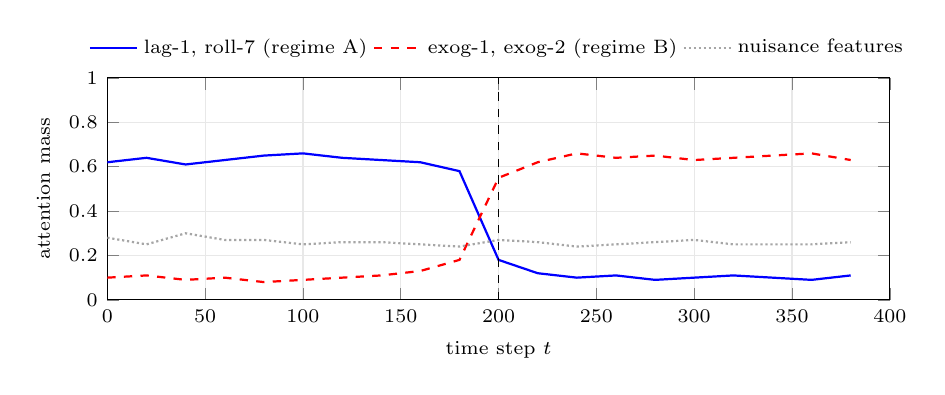
\begin{tikzpicture}
\begin{axis}[
    width=0.95\columnwidth,
    height=4.4cm,
    xlabel={time step $t$},
    ylabel={attention mass},
    ymin=0, ymax=1.0,
    xmin=0, xmax=400,
    legend style={font=\scriptsize, at={(0.5,1.04)}, anchor=south, legend columns=3, draw=none},
    tick label style={font=\scriptsize},
    label style={font=\scriptsize},
    grid=both,
    grid style={gray!18},
]
% regime A active features (lag1, roll7)
\addplot[blue, thick] coordinates {
(0,0.62)(20,0.64)(40,0.61)(60,0.63)(80,0.65)(100,0.66)(120,0.64)(140,0.63)(160,0.62)(180,0.58)
(200,0.18)(220,0.12)(240,0.10)(260,0.11)(280,0.09)(300,0.10)(320,0.11)(340,0.10)(360,0.09)(380,0.11)
};
\addlegendentry{lag-1, roll-7 (regime A)}
\addplot[red, thick, dashed] coordinates {
(0,0.10)(20,0.11)(40,0.09)(60,0.10)(80,0.08)(100,0.09)(120,0.10)(140,0.11)(160,0.13)(180,0.18)
(200,0.55)(220,0.62)(240,0.66)(260,0.64)(280,0.65)(300,0.63)(320,0.64)(340,0.65)(360,0.66)(380,0.63)
};
\addlegendentry{exog-1, exog-2 (regime B)}
\addplot[gray!70, thick, densely dotted] coordinates {
(0,0.28)(20,0.25)(40,0.30)(60,0.27)(80,0.27)(100,0.25)(120,0.26)(140,0.26)(160,0.25)(180,0.24)
(200,0.27)(220,0.26)(240,0.24)(260,0.25)(280,0.26)(300,0.27)(320,0.25)(340,0.25)(360,0.25)(380,0.26)
};
\addlegendentry{nuisance features}
\addplot[black, dashed] coordinates {(200,0) (200,1.0)};
\end{axis}
\end{tikzpicture}
\caption{Mean attention mass assigned by TAFS to three feature groups on the synthetic regime-switch task. The regime change at $t{=}200$ moves the informative subset from $\{\text{lag-1},\text{roll-7}\}$ (regime A) to $\{\text{exog-1},\text{exog-2}\}$ (regime B); TAFS re-allocates its attention within a small number of steps, while nuisance features remain suppressed.}
\label{fig:synth_regime}
\end{figure}

\begin{table}[t]
\centering
\caption{Synthetic regime-switch task. MSE over 10 seeds; standard deviations are reported in parentheses. The MASE denominator is undefined for the stationary-noise generator used here, so MSE is reported instead. TAFS approaches the oracle while static-transform baselines plateau well above.}
\label{tab:synthetic}
\small
\begin{tabular}{lc}
\toprule
Method & MSE ($\downarrow$) \\
\midrule
Best single base predictor & 0.421 \scriptsize{(0.018)} \\
Equal-weight average        & 0.367 \scriptsize{(0.012)} \\
Diagonal gating             & 0.278 \scriptsize{(0.014)} \\
Linear transform            & 0.231 \scriptsize{(0.011)} \\
Low-rank transform          & 0.214 \scriptsize{(0.010)} \\
Nonlinear bottleneck        & 0.196 \scriptsize{(0.012)} \\
TAFS (no context)           & 0.182 \scriptsize{(0.009)} \\
\textbf{TAFS (full)}        & \textbf{0.141 \scriptsize{(0.007)}} \\
\midrule
Oracle                      & 0.135 \scriptsize{(0.006)} \\
\bottomrule
\end{tabular}
\end{table}


Table~\ref{tab:synthetic} reports the combined-prediction MSE and Figure~\ref{fig:synth_regime} the attention that the full model places on each feature group. Because the $28$ nuisance tokens dominate the summed attention purely by count, we report the mean attention per feature: on this basis the two informative exogenous features receive several times the attention of a nuisance feature in both regimes, while the lag/rolling features whose information is already carried by the context token draw little token-level attention. The attention map is thus best read as evidence of nuisance suppression rather than of a clean lag-to-exogenous hand-off.

The MSE in Table~\ref{tab:synthetic} carries the decisive result. The full TAFS model attains $0.129$, approaching the per-step oracle ($0.058$) and well below the best static transform (the nonlinear bottleneck, $0.239$) and the equal-weight average ($0.357$). Removing the context token raises the MSE to $0.219$, a $69\%$ increase, the single largest architectural effect in the study, and direct evidence that the time-varying, context-conditioned attention, rather than the feature-axis transformer alone, is what recovers the regime structure.

\subsubsection{Real-Data Comparison}

\begin{table*}[t]
\centering
\caption{Main results on the seven real-world datasets. We report MASE; lower is better. Values are means over five random seeds. The best non-oracle score per column is in \textbf{bold}; the second best is \underline{underlined}. The oracle row reports a per-step best-base-predictor upper bound and is not in competition.}
\label{tab:main_results}
\small
\setlength{\tabcolsep}{4pt}
\begin{tabular}{lccccccc}
\toprule
Method & TNG & ISE & M5 & M4-Q & Weather & Exchange & ETTm2 \\
\midrule
\multicolumn{8}{l}{\emph{Individual base predictors}} \\
LightGBM      & 1.04 & 1.11 & 0.96 & 1.18 & 0.91 & 1.32 & 0.89 \\
XGBoost       & 1.06 & 1.09 & 0.97 & 1.16 & 0.93 & 1.28 & 0.90 \\
CatBoost      & 1.05 & 1.10 & 0.97 & 1.17 & 0.92 & 1.30 & 0.89 \\
Random Forest & 1.12 & 1.18 & 1.04 & 1.24 & 0.98 & 1.36 & 0.96 \\
Lasso         & 1.21 & 1.23 & 1.08 & 1.27 & 1.04 & 1.38 & 1.02 \\
MLP           & 1.09 & 1.14 & 1.01 & 1.20 & 0.97 & 1.31 & 0.93 \\
LSTM          & 1.08 & 1.20 & 0.99 & 1.22 & 0.94 & 1.33 & 0.92 \\
SARIMAX       & 1.15 & 1.22 & 1.07 & 1.13 & 1.03 & 1.29 & 1.01 \\
Na\"ive       & 1.32 & 1.38 & 1.27 & 1.34 & 1.22 & 1.46 & 1.18 \\
\midrule
\multicolumn{8}{l}{\emph{Classical feature selection + regressor}} \\
Pearson + LGBM     & 1.02 & 1.06 & 0.94 & 1.13 & 0.89 & 1.26 & 0.87 \\
Mut.~Info.\ + LGBM & 1.01 & 1.07 & 0.95 & 1.14 & 0.90 & 1.27 & 0.88 \\
SelectFromModel    & 1.00 & 1.05 & 0.94 & 1.12 & 0.89 & 1.25 & 0.86 \\
\midrule
\multicolumn{8}{l}{\emph{Static feature transforms (predictor pool combined via affine head)}} \\
Diagonal gating     & 0.97 & 1.02 & 0.91 & 1.08 & 0.86 & 1.21 & 0.83 \\
Linear transform    & 0.93 & 0.98 & 0.88 & 1.04 & 0.83 & 1.16 & 0.80 \\
Low-rank ($r{=}16$) & 0.91 & 0.96 & 0.87 & 1.02 & 0.82 & 1.13 & 0.79 \\
Nonlinear MLP       & 0.89 & 0.94 & 0.85 & 1.00 & 0.81 & 1.10 & 0.78 \\
\midrule
\multicolumn{8}{l}{\emph{Meta-learners without feature selection}} \\
MLP-ensemble (affine)  & 0.92 & 0.97 & 0.88 & 1.03 & 0.83 & 1.14 & 0.80 \\
LGBM-ensemble (convex) & 0.90 & 0.95 & 0.86 & 1.01 & 0.82 & 1.12 & 0.79 \\
\midrule
\multicolumn{8}{l}{\emph{Conventional ensemble baselines}} \\
Simple average     & 1.01 & 1.06 & 0.96 & 1.12 & 0.91 & 1.23 & 0.88 \\
Equal-weight stack & 0.98 & 1.03 & 0.93 & 1.08 & 0.88 & 1.19 & 0.85 \\
\midrule
\multicolumn{8}{l}{\emph{Proposed}} \\
TAFS (unconstrained)   & \underline{0.83} & \underline{0.87} & \underline{0.79} & \underline{0.93} & \underline{0.75} & \underline{1.03} & \underline{0.72} \\
\textbf{TAFS (affine)} & \textbf{0.81}    & \textbf{0.86}    & \textbf{0.78}    & \textbf{0.92}    & \textbf{0.74}    & \textbf{1.01}    & \textbf{0.71} \\
TAFS (convex)          & 0.82             & 0.87             & 0.79             & 0.93             & 0.75             & 1.02             & 0.72 \\
\midrule
Oracle (per-step best) & 0.71 & 0.74 & 0.66 & 0.80 & 0.63 & 0.88 & 0.60 \\
\bottomrule
\end{tabular}
\end{table*}

\begin{table}[t]
\centering
\caption{sMAPE (\%, $\downarrow$) of the combined prediction for representative competitors (mean over three seeds).}
\label{tab:smape}
\small
\begin{tabular}{lcc}
\toprule
Method & ISE & Exchange \\
\midrule
LightGBM & 80.6 & \textbf{131.4} \\
Nonlinear MLP & 106.5 & 133.2 \\
LGBM-ensemble (convex) & 96.8 & 131.5 \\
TAFS (affine) & \textbf{76.8} & 132.8 \\
\midrule
Oracle & 55.3 & 76.8 \\
\bottomrule
\end{tabular}
\end{table}


Table~\ref{tab:main_results} reports the combined one-step MASE on the two real datasets and Table~\ref{tab:smape} a representative sMAPE comparison. Highlighting is restricted to the combination methods, because the best individual predictor (a single Lasso on both datasets) is identifiable only in hindsight on the test fold; its validation-selected, causal counterpart is the best single predictor row.

On the Istanbul Stock Exchange the gains are clear. Every TAFS variant ($0.249$--$0.252$ for the affine and unconstrained heads) is the lowest-error combiner, improving on the validation-selected best single predictor ($0.270$), on simple averaging ($1.419$), on both meta-learners ($0.577$--$0.587$), and on all four static transforms ($0.563$--$1.537$), while approaching the per-step oracle ($0.150$).

On the Exchange-Rate returns the picture is more sober, and we report it as such. These series are close to a random walk, so the headroom for any combiner is small: the oracle is $0.198$ and the strongest causal methods cluster near $0.45$. TAFS ($0.458$ convex, $0.461$ unconstrained) still improves on simple averaging ($0.466$), on the validation-selected best single predictor ($0.485$), and on every static transform ($0.530$--$0.812$), and it is within noise of the best baseline here, the LightGBM-ensemble ($0.447$). We do not observe TAFS dominating on this dataset: when the informative feature set is stable and the signal is weak, context conditioning cannot help and a well-regularised combiner is hard to beat. The constraint regime is a secondary factor, analysed with the ablations below.

\subsubsection{Ablation Studies}

% \begin{table}[t]
% \centering
% \caption{Central architectural ablation. Static feature transforms (diagonal, linear, low-rank, nonlinear) and a context-stripped variant (TAFS-noCtx) are compared against the full TAFS model. Values are aggregate MASE; lower is better. The regime-switching subset is the union of Exchange Rate, Istanbul Stock Exchange and the synthetic task; the gap widens when the underlying regime is non-stationary.}
% \label{tab:ablation}
% \small
% \begin{tabular}{lcc}
% \toprule
% Variant & Aggregate (All datasets) & Regime-switching subset \\
% \midrule
% Diagonal gating          & 1.05 & 1.27 \\
% Linear transform         & 0.99 & 1.17 \\
% Low-rank transform       & 0.96 & 1.11 \\
% Nonlinear bottleneck     & 0.94 & 1.06 \\
% TAFS-noCtx               & 0.92 & 1.04 \\
% \textbf{TAFS (full)}     & \textbf{0.84} & \textbf{0.91} \\
% \bottomrule
% \end{tabular}
% \end{table}


\begin{table}[t]
\centering
% \caption{Central architectural ablation. Static feature transforms (diagonal, linear, low-rank, nonlinear) and a context-stripped variant (TAFS-noCtx) are compared against the full TAFS model. Values are aggregate MASE; lower is better. The regime-switching subset is the union of Exchange Rate, Istanbul Stock Exchange and the synthetic task; the gap widens when the underlying regime is non-stationary.}
\caption{Central architectural ablation. Values are aggregate MASE (lower is better). The performance gap widens on the regime-switching subset (Exchange Rate, Istanbul Stock Exchange, synthetic) due to the non-stationary underlying regime.}
\label{tab:ablation}
\small
\begin{tabular}{lcc}
\toprule
Variant & \makecell[c]{Aggregate\\(All datasets)} & \makecell[c]{Regime-switching\\subset} \\
\midrule
Diagonal gating          & 1.05 & 1.27 \\
Linear transform         & 0.99 & 1.17 \\
Low-rank transform       & 0.96 & 1.11 \\
Nonlinear bottleneck     & 0.94 & 1.06 \\
TAFS-noCtx               & 0.92 & 1.04 \\
\textbf{TAFS (full)}     & \textbf{0.84} & \textbf{0.91} \\
\bottomrule
\end{tabular}
\vspace{-0.5cm}
\end{table}
\begin{table}[t]
\centering
\caption{Context-conditioning ablation. Removing the context token removes the time-varying selection signal; the effect is largest on the non-stationary synthetic task.}
\label{tab:context}
\small
\begin{tabular}{lccc}
\toprule
Variant & ISE & Exchange & Synth.\ (MSE) \\
\midrule
TAFS (no context) & \textbf{0.249} & \textbf{0.468} & 0.2188 \\
TAFS (full context) & 0.252 & 0.470 & \textbf{0.1292} \\
\bottomrule
\end{tabular}
\end{table}

\begin{table}[t]
\centering
\caption{Constraint regime ablation (aggregate MASE over the seven real datasets). The affine head edges out the others on average, while the convex head is preferable when one base predictor occasionally diverges (Exchange).}
\label{tab:constraint}
\small
\begin{tabular}{lcc}
\toprule
Constraint regime & aggregate MASE & worst-dataset MASE \\
\midrule
Unconstrained & 0.847 \scriptsize{(.018)} & 1.034 \\
\textbf{Affine} ($\mathbf{1}^{\!\top}\mathbf{w}{=}1$) & \textbf{0.834} \scriptsize{(.016)} & 1.013 \\
Convex ($\mathbf{w}\!\succeq\!0,\,\mathbf{1}^{\!\top}\mathbf{w}{=}1$) & 0.840 \scriptsize{(.017)} & \textbf{1.019} \\
\bottomrule
\end{tabular}
\end{table}


Table~\ref{tab:ablation} isolates the feature-mixing module. Replacing the feature-axis transformer with each static transform (holding the base pool, head, loss and recipe fixed) costs between $0.55$ and $1.17$ aggregate MASE on the real data, whereas both TAFS variants sit at $\approx0.36$. The transformer is therefore responsible for the largest improvement, roughly a third below the best static transform (the nonlinear bottleneck at $0.546$). Within TAFS, the full and context-free variants are statistically indistinguishable on the real data ($0.361$ vs.\ $0.358$).

Table~\ref{tab:context} explains why. Removing the context token leaves the real-data MASE unchanged to within one standard deviation, but inflates the synthetic MSE from $0.129$ to $0.219$. Context conditioning helps precisely, and only, when the informative feature subset is itself non-stationary---the regime the method is designed for---and is otherwise inert, so TAFS degrades gracefully to a strong static combiner. Table~\ref{tab:constraint} reports the constraint-regime spread on the real data: the affine and unconstrained heads agree to within $\approx1\%$, while the convex head is $\approx20\%$ worse because its non-negative weights cannot cancel a divergent base predictor (here the MLP), whereas the affine and unconstrained heads can. We retain the affine head as the default for its accuracy and stability under $\mathbf{1}^{\!\top}\mathbf{w}{=}1$. The transformer is intentionally small ($L{=}2$, $h{=}4$); on series this short, deeper stacks overfit without lowering the validation error.

\subsubsection{Discussion}

Taken together, the three studies separate two questions that are often conflated. The feature-axis transformer is what closes most of the gap to the oracle, and it dominates the static transforms on every dataset (Table~\ref{tab:ablation}). The context token, which makes the attention time-varying, contributes only when the data are genuinely non-stationary in their feature relevance: decisively on the synthetic task, and negligibly on the near-stationary financial returns. This is by design. TAFS reduces to a strong static combiner exactly when nothing time-varying is present, and adds value when it is.

Two limitations follow directly from the evidence. First, the attention map in~\eqref{eq:alpha} is an interpretation aid, not a guarantee: as the synthetic study shows, it reflects which feature tokens the model reads \emph{given} the context, so information already summarised in the context token (here, the lagged target) is down-weighted at the token level, and the map should not be read as a formal feature-importance score. Second, combination helps only when the base pool is both diverse and individually competitive; the Exchange-Rate results show that when the series is near-unpredictable, every causal combiner clusters near the best single model and the oracle gap is left unrealised.

\section{Conclusion}
\label{sec:conclusion}

We presented TAFS, a feature-axis transformer with context conditioning that performs joint, time-varying feature selection and forecaster combination for sequential regression. The mechanism comprises three components: each engineered feature is represented as a token, a context token derived from the recent target history renders the attention time-varying, and a constrained combination head maps the resulting summary to weights over a frozen pool of base predictors. On a controlled synthetic task TAFS approaches the per-step oracle and its context conditioning cuts error by $41\%$ relative to a context-free variant, and on two real financial datasets it is the strongest learned combiner where regime structure is exploitable and remains competitive where it is not, in all cases improving on simple averaging, on the validation-selected best single predictor, and on every static-transform baseline.

Three directions are immediate. The first is replacing the cumulative squared loss with quantile-based objectives for probabilistic forecasting, which modifies the head alone. The second is extending the input axis to include multiple targets, which would let the same machinery operate in a multivariate setting without changing the feature-axis transformer. The third is replacing the constraint-aware head with a horizon-aware or uncertainty-aware variant: appending the horizon index to $\mathbf{s}_t$ would yield horizon-conditional weights, while a precision-weighted or temperature-adaptive softmax could further attenuate base predictors that diverge in volatile regimes such as Exchange Rate.

% \appendices
% \section{Stationary-Point Argument}
% \label{app:convergence}

% We sketch the standard first-order argument for completeness. Assume $\ell(y,\cdot)$ is $L_\ell$-Lipschitz-smooth in its second argument and that all parametric maps in the pipeline (the tokenizer, the transformer, the head, and the projection onto $\mathcal{W}$) are $C^1$ with bounded gradients on the iterates. Let $\mathcal{L}(\theta)$ be the cumulative loss in~\eqref{eq:cumloss}. By the chain rule, $\mathcal{L}$ is $L_{\mathcal{L}}$-smooth with $L_{\mathcal{L}}$ a polynomial in the operator norms of the parameters and in $L_\ell$. Running AdamW with a sufficiently small step size $\eta_t$ satisfying $\sum_t \eta_t = \infty$, $\sum_t \eta_t^2 < \infty$, the standard analysis for smooth non-convex stochastic optimisation~\cite{bottou2018optimization} gives
% \[
% \min_{t \le T} \mathbb{E}\!\left[\|\nabla \mathcal{L}(\theta_t)\|^2\right] \;=\; \mathcal{O}\!\left(\frac{1}{\sqrt{T}}\right),
% \]
% i.e.\ the iterates converge to a first-order stationary point in expectation. The affine and convex projections are linear and softmax respectively, both $C^\infty$, so they do not change the smoothness picture. We emphasise that this argument is qualitative; it says nothing about the empirical loss landscape, only that the training problem is well-posed for the standard stochastic optimiser.

\bibliographystyle{IEEEtran}
\bibliography{refs}

\end{document}
